\documentclass{article}
\usepackage[utf8]{inputenc}
\usepackage{amsmath,graphicx,hyperref,xcolor}

\setlength{\parindent}{0in}
\setlength{\parskip}{1em}

\newcommand{\purple}[1]{{\color{purple} #1}}

\usepackage{fancyhdr}
\rhead{}

\pagestyle{fancy}
\lhead{Physics 374B Midterm}
\rhead{Fall 2020}
\cfoot{\thepage}

\begin{document}

Name: \makebox[2in]{\hrulefill\purple{SOLUTION}\hrulefill}

\vspace{0.5in}

\begin{itemize}
    \item Due by 3pm Monday to the folder outside Darla's office (RNS 236).
    \item Number your pages. Put your name on each page.
    \item Work on your own. You may reference your notes and the book. 
    \item Each bullet is worth the same number of points. Some are more difficult than others.
    \item I have confidence in you!
\end{itemize}

\vfill

I pledge my honor that on this examination I have neither given nor received assistance not explicitly approved by the professor and that I have seen no dishonest work \makebox[2in]{\hrulefill}

\vspace{0.5in}

I have intentionally not signed this pledge \makebox[2in]{\hrulefill}

\newpage

\section*{Problem 1}

There are 13 physicist videos on Moodle from you and your classmates. How many had you watched before starting this midterm?

What are three things you found notable?

\newpage

\section*{Problem 2}

A spherical ball of radius $r$ rolls without slipping in a half-pipe of radius $R$.

\begin{itemize}
    \item Write down the Lagrangian for this system in terms of two variables: the ball's position and its rotation. Make sure the meaning of each variable is clearly marked on your diagram.
    
    Hint: rotational kinetic energy takes the form $T_{rot} = \tfrac{1}{2} I \omega^2$ where $\omega$ is the angular velocity and $I = \tfrac{2}{5} m r^2$ is the moment of inertia for a sphere rotating around its center.
    \item Write down a constraint to describe the relationship between your two variables. Where does this come from?
    \item Use the Euler-Lagrange equation and a Lagrange multiplier to write down the equations of motion for this system. 
    $$
    \frac{\partial \mathcal{L}}{\partial x} + \lambda \frac{\partial g}{\partial x} = \frac{d}{dt} \frac{\partial \mathcal{L}}{\partial \dot{x}}
    \quad\quad\text{for each coordinate $x$}
    $$
    \item Solve the equation of motion for the case of small motions near the bottom of the half-pipe.

    Hint: When $\xi$ is small, $\sin\xi \approx \xi$
    \item Find the value of your Lagrange multiplier. What is its physical significance?
    \item Discuss the behavior of this system in the limiting cases $r \rightarrow 0$ and $r \rightarrow R$.
    \item How does your solution compare to the behavior of a simple pendulum?
    
    Hint: for small oscillations, a pendulum oscillates with frequency $\sqrt{\frac{g}{\ell}}$
\end{itemize}

\newpage

\section*{Problem 3}

A soap bubble is enclosed by three rigid wires (each length $L$) and a flexible string (length $\ell > L$) as shown. The wires form three sides of a square. The surface tension of the bubble pulls the string taut to minimize the enclosed area.

\begin{figure}[h]
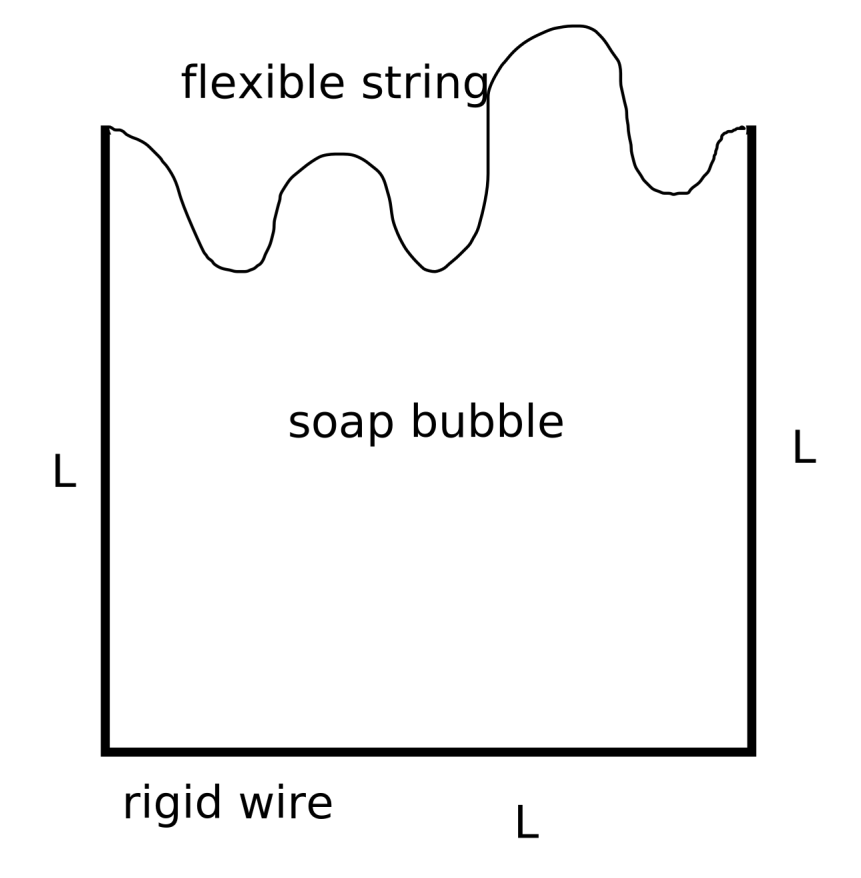
\includegraphics[width=4cm]{string-bubble.png}
\centering
\end{figure}

\begin{itemize}
    \item Write down an expression for the enclosed area using rectangular coordinates $x$ and $y$.
    \item Write down an expression for the relevant constraint.
    \item Use the Euler-Lagrange equation to minimize the enclosed area. 
    Show that the resulting differential equation is:
    $$
    \frac{dy}{dx} = \frac{ \sqrt{ \lambda^2 - \left( y - y_0 \right)^2 } }{ y - y_0 }
    \quad\quad\text{where $y_0$ and $\lambda$ are constants}
    $$
    Hint: when $f(y, y', x)$ doesn't include $x$, the EL equation can be written: 
    $$
    \frac{\partial f}{\partial y} - \frac{d}{dx} \frac{\partial f}{\partial y'} = 0
    \quad\quad\rightarrow\quad\quad
    f - y' \frac{\partial f}{\partial y'} = \text{constant}
    $$
    \item Separate and solve the differential equation. 
    
    Hint: Try the substitution $\sin u = \tfrac{y - y_0}{\lambda}$
    \item There is a common name for the resulting curve. What is it? (For example: catenary, circle, cosine, ellipse, hyperbola, parabola, etc)
    \item Draw a diagram of the solution. Based on that diagram, write down an equation to solve for each undetermined constant.
    \item Let $L=10\,\text{cm}$ and $\ell=20\,\text{cm}$. Solve numerically for the values of each undetermined constant. You may use Mathematica or Wolfram Alpha on this part.
    
\end{itemize}

\newpage
\section*{For Reference}

Taylor does not cover this usage of Lagrange multipliers. 

Suppose you have a quantity $A$ defined as:
$$
A = \displaystyle\int_{x_0}^{x_1} f(y, y', x) \; dx
\quad\quad\text{where $y' = \tfrac{dy}{dx}$}
$$
Suppose further that $y(x)$ is subject to a constraint of the form:
$$
\ell = \displaystyle\int_{x_0}^{x_1} g(y, y', x) \; dx
\quad\quad\text{where $\ell$ is fixed}
$$
You're looking for $y(x)$ that extremizes the value of $A$ while respecting the constraint. The solution is obtained by extremizing $A^*$:
$$
A^* = \displaystyle\int_{x_0}^{x_1} f(y, y', x) + \lambda \; g(y, y', x) \; dx
$$
Where $\lambda$ is an undetermined constant.

\newpage

We haven't used numerical solvers much. Here's a quick example:

\begin{figure}[h]
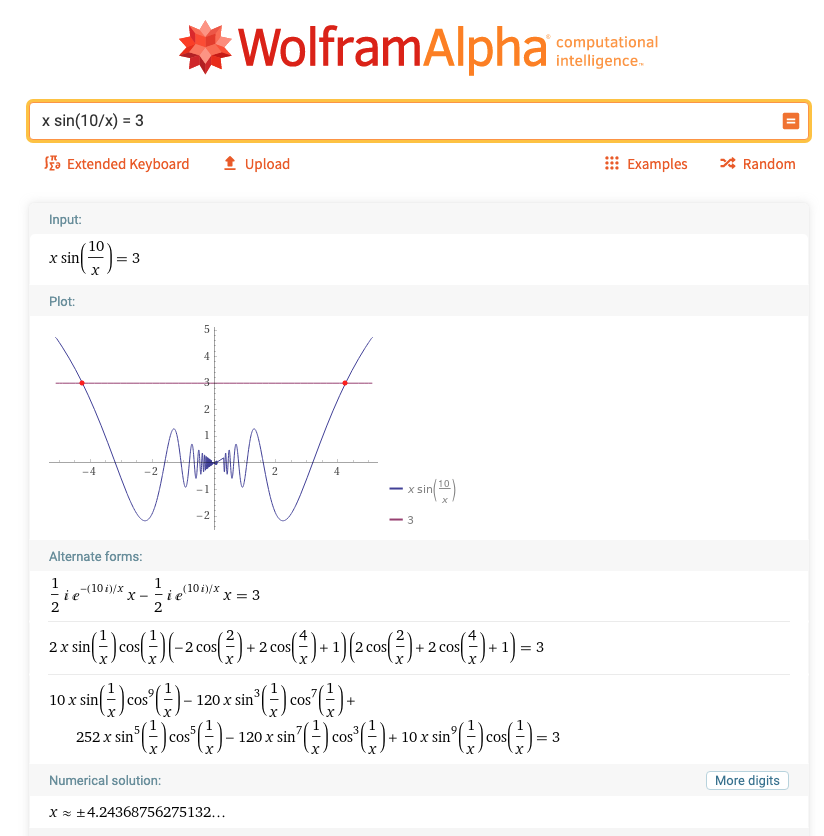
\includegraphics[width=12cm]{wolfram-solver-example.png}
\centering
\end{figure}

\newpage

\section*{Problem 2 Solution}


\begin{figure}[h]
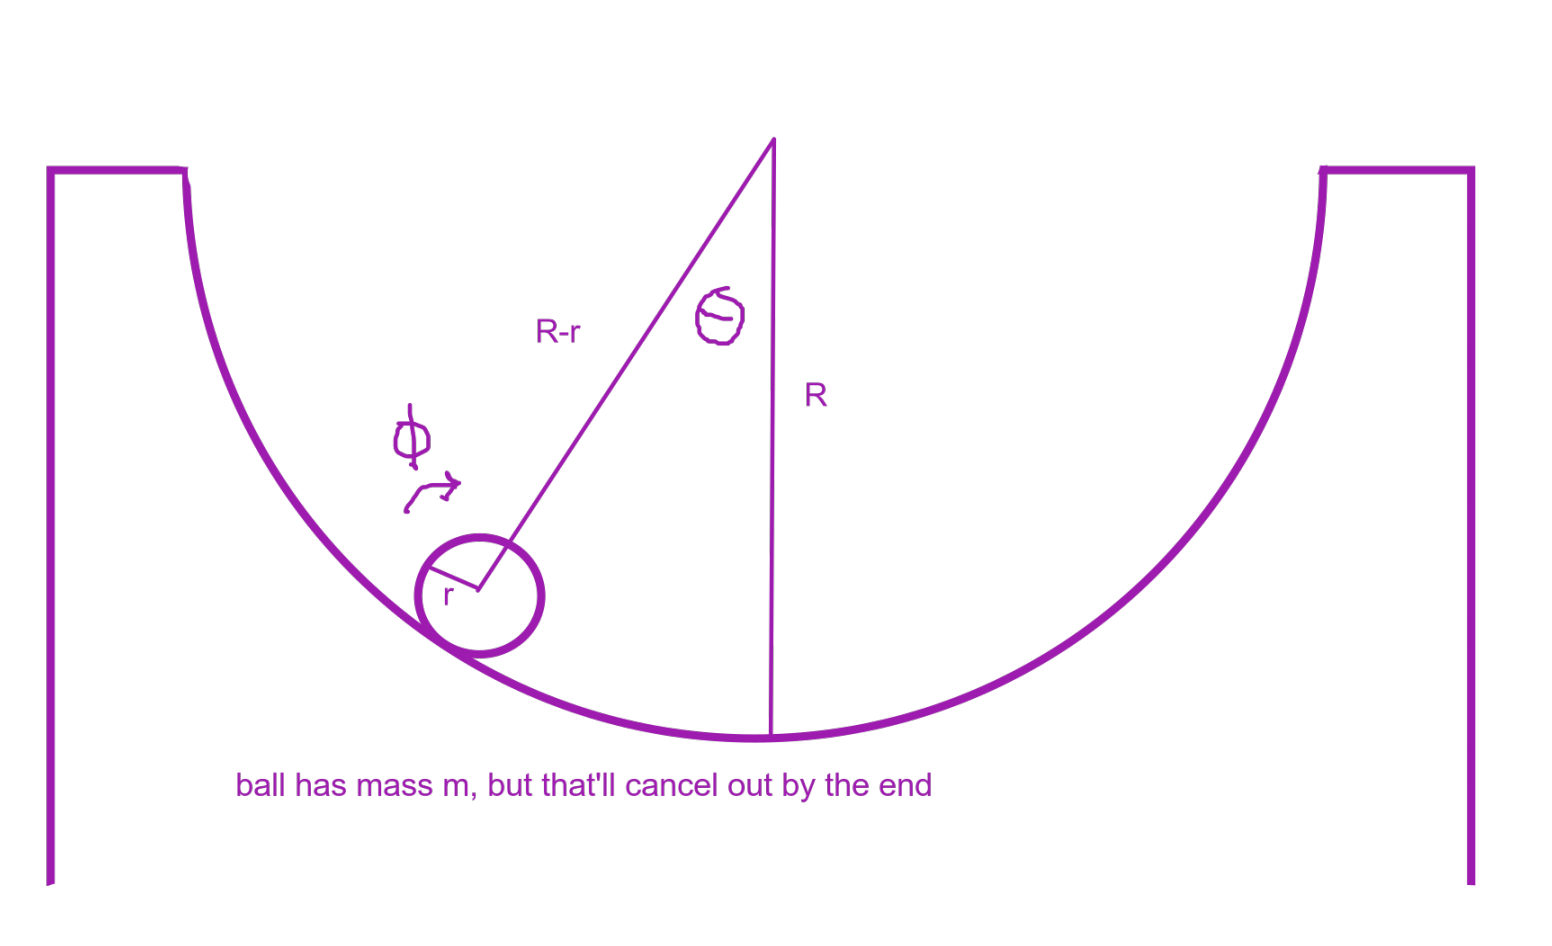
\includegraphics[width=10cm]{half-pipe.png}
\centering
\end{figure}


\purple{
The center of mass of the ball is always a distance $R-r$ from the center of the half-pipe, so it's convenient to track the position of the ball in terms of an angle $\theta$. We use another angle, $\phi$, to track its rotation. Then the Lagrangian for this system can be written:
$$
\mathcal{L} = T_{trans} + T_{rot} - U_{grav} = \tfrac{1}{2} m (R-r) \dot{\theta}^2 + \tfrac{1}{2} I \dot{\phi}^2 + mg(R-r)\cos\theta
$$
The angles $\theta$ and $\phi$ are related by the rolling-without-slipping condition. It's a bit tricky to picture, since we're rolling over a curved surface. If the ball does a full rotation, it will have covered more ground than $2\pi r$, since the surface (in essence) rises up to meet it. You can think of this in terms of radius, by matching up the center of mass instead of the point that rolls. Or you can think of it in terms of angle, where the ball is affected by both $\theta$ and $\phi$. Either way we end up with:
$$
r \phi = (R-r) \theta
\quad\quad\text{or, to put it in the proper form,}\quad\quad
r\phi - (R-r) \theta = 0
$$
Plugging into the Euler-Lagrange equation, we get two equations of motion:
\begin{align*}
    -mg(R-r)\sin\theta - \lambda (R-r) &= m (R-r)^2 \ddot{\theta} \\ 
    0 + \lambda r &= I \ddot{\phi}
\end{align*}
Taking the time derivative of the constraint, we also get:
$$
r \phi = (R-r) \theta
\quad\quad\rightarrow\quad\quad
r \dot{\phi} = (R-r) \dot{\theta}
\quad\quad\rightarrow\quad\quad
r \ddot{\phi} = (R-r) \ddot{\theta}
$$
After a bit of algebra, we can rearrange the two equations of motion (and the constraint) to get:
$$
-mg (R-r)\sin\theta = \left( m (R-r)^2 + I \tfrac{(R-r)^2}{r^2} \right) \ddot{\theta}
$$
Or, noting $I = \tfrac{2}{5}mr^2$:
$$
\ddot{\theta} = -\frac{5}{7} \frac{ g }{R - r}\sin\theta
$$
In the limit of small oscillations, $\sin\theta \rightarrow \theta$, in which case the solution is:
$$
\theta(t) = A \cos \left( \omega t - \theta_0 \right)
\quad\quad\text{where}\quad\quad
\omega^2 = \frac{5}{7} \frac{g}{R-r}
$$
And the constants $A$ and $\theta_0$ are dictated by the initial conditions.

When $r \rightarrow R$, the acceleration is zero. The ball sits snugly in the half-pipe.

In the limit $r \rightarrow 0$, the acceleration is:
$$
\ddot{\theta} \rightarrow -\frac{5 g}{7 R} \sin\theta
\quad\quad\text{or}\quad\quad
\omega^2 \rightarrow \frac{5}{7} \frac{g}{R}
$$
This is a somewhat slower oscillation than we see with a simple pendulum ($\omega^2=\frac{g}{R}$). For the pendulum, all of the kinetic energy is translational. The ball is working with the same amount of gravitational potential energy, but some of it has to power the rotation, so the translation is slower. 

We can also go back and solve for $\lambda$. Plugging our expression for $\ddot{\theta}$ back into our equation of motion we get:
$$
-mg(R-r)\sin\theta - \lambda R = -m (R-r)^2 \frac{5}{7} \frac{ g }{R - r}\sin\theta
$$
Or:
$$
\lambda = -\tfrac{2}{7} m g \sin\theta
$$
In other words, $\lambda$ is the difference between the gravitational force on the ball and its acceleration. Physically, this manifests as a frictional force which enforces the rolling without slipping condition. It's the difference between the acceleration felt by a slipping mass ($mg\sin\theta$) and that seen above.

\newpage

Denote the position of the string $y(x)$. Then the enclosed area is given by:
$$
A = \displaystyle\int_{0}^{L} y \; dx
$$
The constraint is that the length of the string is fixed. As we saw for the hanging chain, the constraint there is:
$$
\ell = \displaystyle\int_{0}^{L} \sqrt{1 + y'^2} \; dx
$$
Where $y' = \tfrac{dy}{dx}$ and  $\ell$ is fixed.

Combining the two, we get:
$$
A^* = \displaystyle\int_{0}^{L} \underbrace{ y + \lambda \sqrt{1 + y'^2} }_{f(y, y', x)}\; dx
$$
Note that $\lambda$ above is constant, unlike in the previous problem.

To find a minimum area that respects our constraint, we plug into the Euler-Lagrange equation. Since $f$ does not depend explicitly on $x$, we can use the shortcut from the hint. We end up with:
$$
y + \lambda \sqrt{1 + y'^2} - y' \lambda \frac{y'}{\sqrt{1 + y'^2}} = y_0 \quad\text{(constant)}
$$
Then a bit of algebra to get rid of the square roots and solve for $y'$:
\begin{align*}
    y + \lambda \sqrt{1 + y'^2} - y' \lambda \frac{y'}{\sqrt{1 + y'^2}} &= y_0 \\
    y\sqrt{1 + y'^2} + \lambda (1 + y'^2) - \lambda y'^2 &= y_0 \sqrt{1 + y'^2} \\
    (y - y_0) \sqrt{1 + y'^2} &= -\lambda \\
    (y - y_0)^2 (1 + y'^2) &= \lambda^2 \\
    (y - y_0)^2 y'^2 &= \lambda^2 - (y - y_0)^2 \\
    y' &= \frac{ \sqrt{ \lambda^2 - (y - y_0)^2 } }{y - y_0}
\end{align*}
Then we separate and finagle our square root to the form $\sqrt{ 1 - \text{stuff}^2}$ in anticipation of a $u$ substitution.
\begin{align*}
    \frac{dy}{dx} &= \frac{ \sqrt{ 1 - \left( \frac{y - y_0}{\lambda} \right)^2 } }{\left( \frac{y - y_0}{\lambda} \right)} \\
    \frac{\left( \frac{y - y_0}{\lambda} \right)}{\sqrt{ 1 - \left( \frac{y - y_0}{\lambda} \right)^2 }}dy &= dx \\
\end{align*}
Then let $\sin u = \tfrac{y - y_0}{\lambda}$, so $\cos u \, du = \frac{dy}{\lambda}$ (so $dy = \lambda \cos u \, du$), and integrate:
\begin{align*}
    \int \frac{\left( \frac{y - y_0}{\lambda} \right)}{\sqrt{ 1 - \left( \frac{y - y_0}{\lambda} \right)^2 }} dy &= \int dx \\
    \int \frac{ \sin u }{\sqrt{ 1 - \sin^2 u^2 }} \lambda \cos u \, du &= \int dx \\
    \lambda \int \sin u \; du &= \int dx \\
    -\lambda \cos u &= x - x_0 \\
\end{align*}
Where $x_0$ is a constant of integration. To get back from $u$ to $y$, we then need to note:
$$
\sin u = \sqrt{ 1 - \cos^2 u } = \sqrt{ 1 -  \left( \frac{y - y_0}{\lambda} \right)^2 }
$$
So:
\begin{align*}
    -\lambda \cos u &= x - x_0 \\
    -\lambda \sqrt{ 1 -  \left( \frac{y - y_0}{\lambda} \right)^2 } &= x - x_0 \\
    \lambda^2 &= (x - x_0)^2 + (y-y_0)^2 \\
\end{align*}
In other words, the string is pulled into the arc of a circle. The radius of the circle is $\lambda$, and the center of the circle is at $(x_0, y_0)$.
\begin{figure}[h]
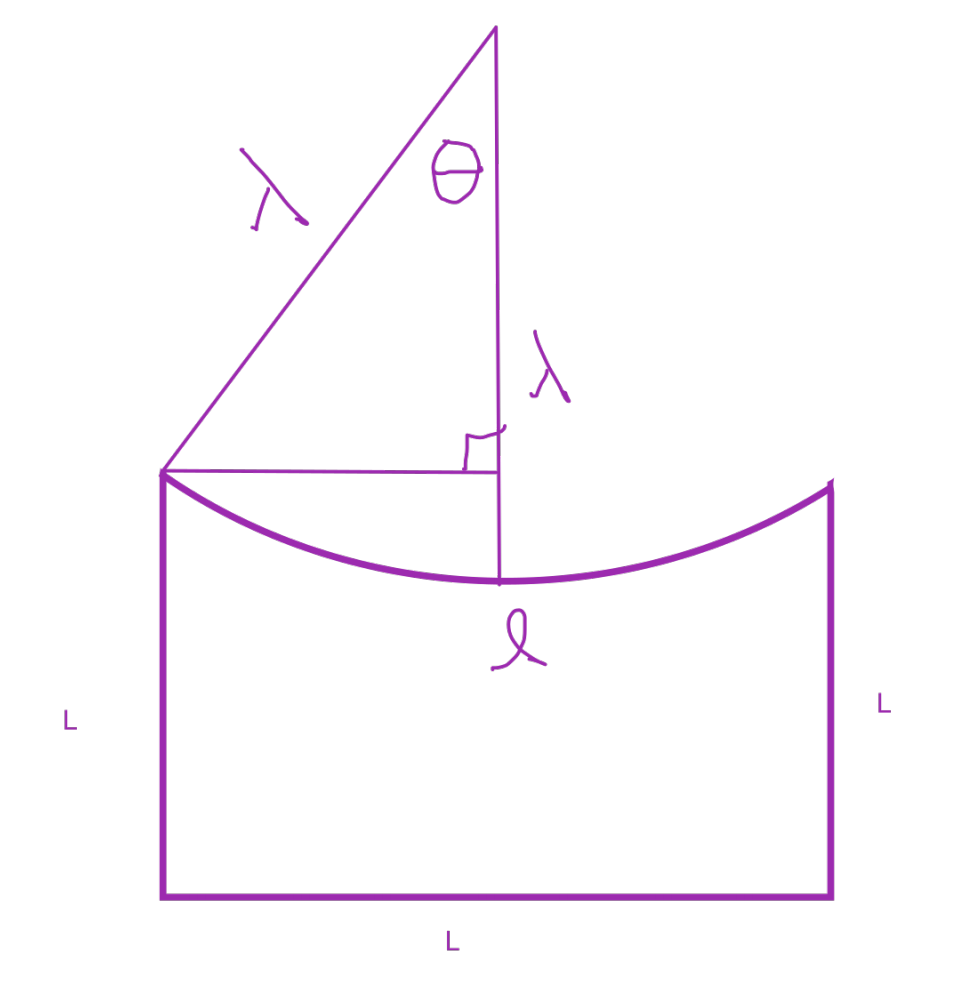
\includegraphics[width=10cm]{circular-arc.png}
\centering
\end{figure}
From this diagram, we can write down a few relationships between our quantities, with the help of an arc angle $\theta$. 

From the length of the arc:
$$
\frac{\ell}{2} = \lambda \theta
$$
From the height of the center of the circle:
$$
y_0 = L + \lambda \cos\theta
$$
And we can see $x_0$ must be in the middle by symmetry:
$$
x_0 = \frac{L}{2} = \lambda \sin\theta
$$
We can combine the first and third expressions to end up with an equation where $\lambda$ is the only unknown:
$$
\frac{L}{2} = \lambda \sin \frac{\ell}{2\lambda}
$$
This cannot be solved directly, but it can be solved numerically. Using the quantities given:
$$
\frac{10\, \text{cm}}{2} = \lambda \sin \frac{20\, \text{cm}}{2 \lambda}
\quad\quad\rightarrow\quad\quad
\lambda \approx 5.28 \, \text{cm}
\quad\quad\text{per Wolfram Alpha}
$$
Then we can plug that in to get:
$$
\theta = 1.90 \, \text{rad}
\quad\quad\text{and}\quad\quad
y_0 = 8.31 \, \text{cm}
$$
You'll notice that the center of the circle is below the tips of the wires... this is a typo on my part. I should have used $\ell=15\, \text{cm}$.

Imagine a circle of diameter $L = 2\lambda$ between the wires. It just barely touches them. A string following its curve would then have a length of $\pi \lambda$, half the diameter of that circle.

For shorter $\ell$, we can decrease $\theta$ (and increase $\lambda$) to get a straighter string. As $\ell \rightarrow L$, $\theta \rightarrow 0$ and $\lambda \rightarrow \infty$.

But we can't really do the opposite for longer $\ell$. The only way to get $20 \, \text{cm}$ of string on a circular arc between wires $10 \, \text{cm}$ apart is to backtrack and/or let the circle extend outside the wires. The math works just fine, but the situation is not physical.

Full credit for good attempts on this part, and an extra point if you caught my mistake

}






\end{document}
